\documentclass[11pt, paper=a4]{scrartcl}

% CONFIG
\newcommand{\exptitle}{Optical pumping}       % long name of experiment 
\newcommand{\exptitleshort}{Optical pumping} % short name of experiment
\newcommand{\expdate}{11.04.2016}           % date of experiment
\newcommand{\exptutor}{Dominik Schomas}

% PACKAGES + MODIFICATIONS
%\usepackage[ngerman]{babel} %standard language stuff
\usepackage[T1]{fontenc}
\usepackage[utf8]{inputenc}
\usepackage{textgreek}

\usepackage{soul} %better underline
\setul{2pt}{.4pt} %set underline 2 pts below text and thickness to .4pt

\usepackage[fleqn]{amsmath}  % math
\usepackage{amssymb}

\usepackage{graphicx} %graphics
\usepackage{float} 

\usepackage[automark,headsepline]{scrlayer-scrpage} %headings
\pagestyle{scrheadings}
\ihead{\exptitleshort}
\ohead{\pagemark}
\cfoot{}

\usepackage{hyperref}
\hypersetup{
    unicode=true,          % non-Latin characters in Acrobat’s bookmarks
    pdftoolbar=true,       % show Acrobat’s toolbar?
    pdfmenubar=true,       % show Acrobat’s menu?
    pdffitwindow=false,    % window fit to page when opened
    pdfstartview={FitH},   % fits the width of the page to the window
    pdfnewwindow=true,     % links in new window
    colorlinks=true,       % false: boxed links; true: colored links
    linkcolor=blue,       % color of internal links (change box color with linkbordercolor)
    citecolor=green,       % color of links to bibliography
    filecolor=magenta,     % color of file links
    urlcolor=blue          % color of external links
}

\usepackage[labelfont=bf]{caption} % bold captions

\usepackage{chngcntr} % change behaviour of counters in different environments
\counterwithin{figure}{section}  % number figures per section
\numberwithin{equation}{section} % number equations per section
\numberwithin{table}{section}    % number tables per section

\usepackage{enumerate} % better way to config enumerates

\setcounter{tocdepth}{2} % table of contents depth

\setlength{\parindent}{0pt} % no indent on new paragraph

\usepackage{pdfpages} % include pdf files

\usepackage[nottoc,numbib]{tocbibind} % bibliography in TOC

% NEW COMMANDS
\newcommand{\refeq}[1]{\overset{\text{\eqref{#1}}}{=}}

% DOCUMENT SETTINGS

\title{\exptitle}
\subtitle{}
\author{}
\date{\expdate}

% DOCUMENT
\begin{document}

\hypersetup{pageanchor=false} %stop page numbering (hyperref) to prevent for double page numers
\newcommand{\HRule}{\rule{\linewidth}{0.5mm}}
\begin{titlepage}
\begin{center}
  \textsc{\Large Fortgeschrittenen Praktikum II }\\[0.5cm]
  \HRule \\[0.4cm]
  { \huge \bfseries \exptitle}\\
  \HRule \\[0.5cm]
  \large \expdate\\[0.5cm]  
  Benjamin Winkelmann \\
  Peter Spalthoff \\
  \vspace{10pt}
  \large 
  Tutor: \exptutor \\[3cm]
  \vfill
  \normalsize
\end{center}
\end{titlepage}
\thispagestyle{empty}



\pagenumbering{Roman}
\setcounter{page}{1}


\section{Abstract}
Optical pumping between Zeeman states of rubidium isotopes $^{87}$Rb and $^{85}$Rb that are split up by well controlled magnetic fields allows for the precise calculation of the earths magnetic field, hyperfine constants $A$ of the two isotopes as well as the relaxation time of the polarized states. The resulting hyperfine constants were calculated as
\begin{align}
	A_{^2S_{\nicefrac{1}{2}}}(^{87}Rb)&=\unit{(14.61\pm0.13)}{\micro\electronvolt}\\
	A_{^2S_{\nicefrac{1}{2}}}(^{85}Rb)&=\unit{(4.50\pm0.08)}{\micro\electronvolt}\\
	A_{^2P_{\nicefrac{1}{2}}}(^{87}Rb)&=\unit{(1.52\pm0.18)}{\micro\electronvolt}
\end{align}
The hyperfine constant $A_{^2P_{\nicefrac{1}{2}}}(^{85}Rb)$ could not be calculated since the relevant peaks could not be separated with the set-up.
The earths' magnetic field components were calculated to be
\begin{align}
	B_v&=\unit{(37.1\pm1.4)}{\micro T}\\
	B_h&=\unit{(2.36\pm 0.21)}{\micro T}
\end{align}
Of the two methods used to calculate the relaxation times, only the Dehmelt method produced a reasonable result for the relaxation time:
\begin{equation}
T_R=\unit{(4.8\pm1.5)}{ms}
\end{equation}
\tableofcontents

\newpage
\listoffigures
\thispagestyle{empty}

\newpage
\hypersetup{pageanchor=false} %stop page numbering (hyperref) to prevent for double page numers

\clearpage
\pagenumbering{arabic}
\setcounter{page}{1}

\section{Goal of the experiment}
In this experiment, the process of optical pumping will be used to precisely measure properties of Rubidium atoms such as the hyperfine constant $A$ via absorption measurements. In addition to that, relaxation times of the induced pumped states as well as external magnetic fields will also be measured by observing the effect of magnetic fields, applied through Helmholtz coils, high frequency radio waves and variations in the laser intensity.
\section{Physical principles}
\subsection{Hyperfine structure and Zeeman splitting}
This section is based on the detailed elaborations in \cite{staatsex}.\\
The fine structure levels of the atomic spectrum, which splits the basic levels into sub-levels due to spin-orbit interaction, can be shown to be split into even finer levels, whose energetic distances are roughly three orders of magnitude smaller than those of the fine structure. This is called the 'hyperfine structure' and is mainly caused by the interaction of the nuclear magnetic dipole and quadrupole moment and the magnetic field of the shell electrons. Its structure for the two Rubidium isotopes that are used in this experiment can be seen in figure \ref{fig:hyperfinestructure}.\\

As the nucleus is charged and, expressed as the nuclear spin $\vec{I}$, has angular momentum, it also has a magnetic moment, which is $\vec{\mu}_I=\frac{g_I\mu_K}{\hbar}\vec{I}$, where $g_I$ is the g-factor of the nucleus and $\mu_K$ is the nuclear magneton. 

With the total angular momentum of the electrons $\vec{J}$, the total angular momentum of the atom can be written as

\begin{equation}
\vec{F}=\vec{J}+\vec{I},\qquad \lvert I-J\rvert\le F \le I+J
\end{equation}

The energy difference between hyperfine structure levels can then shown to be

\begin{equation}
\Delta E_{HFS}=-\vec{\mu}_I\cdot\vec{B}_J=\frac{A}{2}(F(F+1)-J(F+1)-I(I+1))
\end{equation}

where $A=\frac{g_I\mu_KB_J}{\sqrt{J(J+1)}}$ is the hyperfine constant. Neighboring levels thus have an energy difference of

\begin{equation}
\Delta E_{HFS}(F+1)-\Delta E_{HFS}(F)=A(F+1)
\label{eq:hfslevels}
\end{equation}

This structure for the rubidium isotopes used in this experiment can be seen in figure \ref{fig:hfslevels}.\\

\begin{figure}[H]
\centering
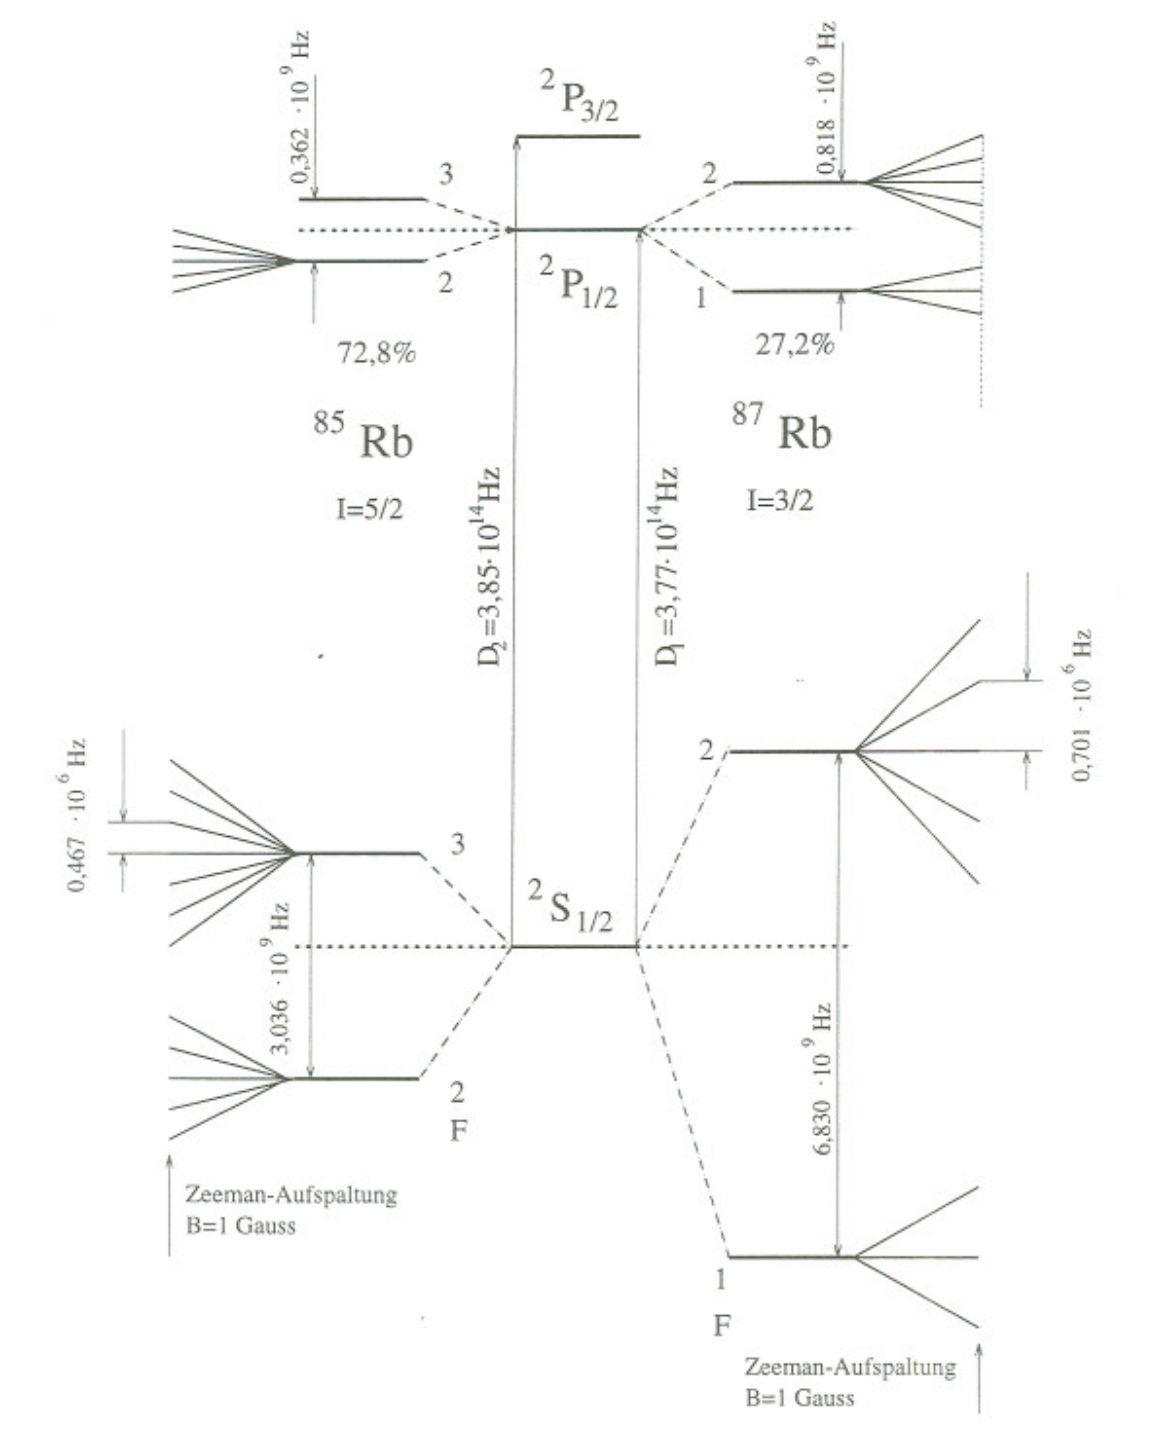
\includegraphics[width=1.0\linewidth]{graphics/hyperfinestructure}
\caption[Hyperfine structure of Rubidium]{The hyperfine structure of the two isotopes of Rubidium used in the experiment. The hyperfine levels in turn are split due to the Zeeman effect caused by an external field of $B=1$ G. \cite{staatsex}}
\label{fig:hyperfinestructure}
\end{figure}

\begin{figure}[H]
\centering
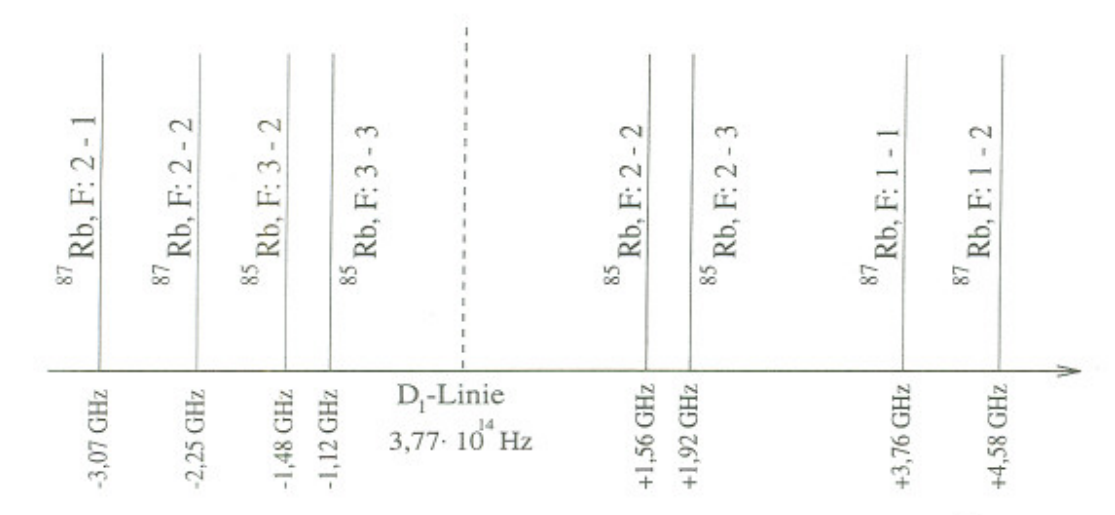
\includegraphics[width=1.0\linewidth]{graphics/hfslevels}
\caption[Hyperfine structure energies]{Energies of a set of hyperfine levels of the two isotopes used in the experiment. \cite{staatsex}}
\label{fig:hfslevels}
\end{figure}

These hyperfine levels can in turn be split into $2(F+1)$ sub-levels in the presence of an external magnetic field. The according quantum number is $-F\le m_F\le F$. As long as the magnetic field is weaker than the spin-orbit coupling or, in other terms, $g_J\mu_BB_0\ll A$, this is called the Zeeman effect. The effect for larger fields, where the spin-orbit coupling is disrupted, is called Paschen-Back effect.\\
For the Zeeman effect, the energy difference of the levels is
\begin{equation}
\Delta E_{Zeeman}=\frac{g_J}{2(I+\frac{1}{2})}\mu_BB_0
\label{eq:zeemanlevels}
\end{equation}

\subsection{Optical pumping}
In general, pumping refers to constantly transferring electrons into higher energy levels until significantly more electrons are in the higher than in the lower state. This is called population inversion.\\
In the case of this experiment, this is done using a laser diode. As the goal is to examine magnetic fields using the Zeeman splitting, a way must be found to create population inversion within a single non-degenerate hyperfine structure level. Normally, electrons are equally distributed between said levels.\\
The selection rules for transitions
\begin{equation}
\begin{aligned}
\Delta F&=0,\pm 1 \qquad (F=0\nleftrightarrow F=0)\\
\Delta m_F&=0,\pm 1
\end{aligned}
\end{equation}

allow for a convenient way to change that. If only $\sigma^+$-polarized light is used, only transitions with $\Delta m_F=+1$ are caused. Since the following decay is random within the bounds of the transition rules, the laser will pump all electrons into the $^2S_{1/2}$ state with $m_F=+2$, $F=2$ for $^{87}Rb$ and $m_F=+3$, $F=3$ for $^{85}Rb$. Figure \ref{fig:zeemanpumping} illustrates this for two exemplary transitions.\\
Mathematically, this process can be described as 
\begin{equation}
\left(\frac{dn}{dt}\right)_P=\frac{N-n}{T_P}
\label{eq:pumpingtime}
\end{equation}
where $n$ is difference of the levels in the two-level system, $N$ the overall number of atoms in the system and $T_P$ the characteristic pumping time of the system.
\begin{figure}[h]
\centering
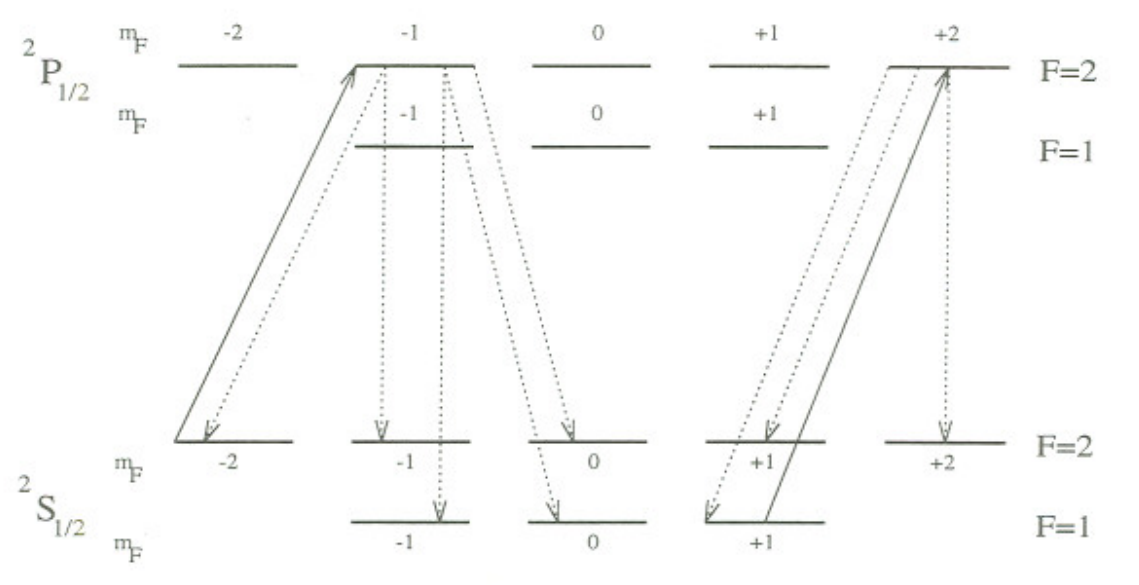
\includegraphics[width=1.0\linewidth]{graphics/zeemanpumping}
\caption[Optical pumping]{Optical pumping for $^{87}Rb$. The $\sigma^+$ polarized light can only cause transitions with $\Delta m_F=+1$, thus achieving the desired pumping effect.}
\label{fig:zeemanpumping}
\end{figure}
\subsection{Relaxation processes}
The desired pumping effect is counteracted mainly by three relaxation effects:
\paragraph{Diffusion to the wall:}
Upon hitting the glass containment, the rubidium atoms may lose their polarization. This process is inhibited by a buffer gas, which limits the mean free path of the atoms.
\paragraph{Collisions with the buffer gas:}
The rubidium atoms may use their polarization due to collisions with the buffer gas. The cross section of this event depend highly on what kind of gas is used. Best results are achieved with noble gases - in the case of this experiment, krypton was used.
\paragraph{Spin exchange}
When rubidium atoms collide, they may interchange their spins. While the overall polarization is preserved, the decoupling of nuclear and electron spins lead to a faster relaxation time. Much more detailed elaborations can be found in \cite{happer}.\\

Overall, the relaxation can be described by the following differential equation
\begin{equation}
\left(\frac{dn}{dt}\right)_R=-\frac{n}{T_R}
\label{eq:relaxationtime}
\end{equation}
where $T_R$ is the characteristic relaxation time. A value of $T^{theo}_R=6.5$ ms is given in \cite{staatsex}. The overall process of polarization orientation is thus the sum of equations \ref{eq:pumpingtime} and \ref{eq:relaxationtime}:
\begin{equation}
\left(\frac{dn}{dt}\right)_O=\left(\frac{dn}{dt}\right)_P+\left(\frac{dn}{dt}\right)_R=\frac{N}{T_P}-n\left(\frac{1}{T_P}+\frac{1}{T_R}\right)
\end{equation}

The solution of this equation is an exponential
\begin{equation}
n(t)\propto e^{-\frac{t}{\tau}}
\label{eq:orientationexponential}
\end{equation}

where $\tau=\frac{1}{T_P}+\frac{1}{T_R}$.
\subsection{Larmor precession of the spin}

\subsection{The laser diode}


\input{analysis}


\newpage
\bibliographystyle{plain}
\bibliography{refs}
\begin{thebibliography}{9}
	\bibitem{staatsex}
	Baur, Clemens. "Einrichtung des Versuchs \emph{Optisches Pumpen mit Laserdioden}."
	Zulassungsarbeit, Freiburg 1997
	\bibitem{happer}
	Happer, William. "Optical pumping."
	\ul{Reviews of Modern Physics} 44.2 (Apr. 1972): 170-238
\end{thebibliography}


\end{document}
